\subsection{Stochastic Games}
We consider a graph-based game formalism between two players. A
(2.5-player) \emph{stochastic game} (SG) is a tuple $\sg = \langle S,
\iota, \Act, P \rangle$.  The set of \emph{states} $S = S_\pOne \cup
S_\pTwo$ is partitioned into a set $S_\pOne$ of (controlled)
$\pOne$-states and a set $S_\pTwo$ of (uncontrolled)
$\pTwo$-states. $\iota \in S_\pTwo$ is the \emph{initial state}, $\Act$ is a
finite set of \emph{actions}, and $P\colon S \times \Act \rightarrow
\Distr(S)$ is the \emph{transition function}. For simplicity of
exposition, we shall assume w.l.o.g. that controlled and uncontrolled
states alternate. Thus, $P$ is defined by two partial transition functions:
$P_\pOne\colon S_\pOne \times \Act \rightarrow \Distr(S_\pTwo)$,
$P_\pTwo\colon S_\pTwo \times \Act \rightarrow \Distr(S_\pOne)$. We
identify the available actions\footnote{We explicitly allow to model
unavailable actions, e.g., we can model that a door can only opened
when close enough to the door.} as $\EnAct(s) \eqdef \{ \act \mid
P(s,\act) \neq \bot \}$. States without available actions, i.e.,
states with $\EnAct(s) = \emptyset$ are called \emph{terminal states}.
A SG is finite, if its state space is finite.  The \emph{successor
states} of a state $s$ and an (enabled) action $\act$ is the set of
states that are reached from $s$ within one step with a positive
transition probability, i.e., $\Succ(s,\act) \eqdef \{ s' \mid
P(s,\act)(s')>0 \}$, and $\Succ(s) \eqdef\bigcup_{\act \in \EnAct(s)}
\Succ(s,\act)$.


\begin{figure}
\centering
\begin{tikzpicture}
	\node[sstate] (s0) {$s_0$};
	\node[astate,right=of s0] (s1) {$s_1$};
	\node[sstate,below=of s1] (s2) {$s_2$};
	
	\node[tstate,right=1.4cm of s1] (target) {$\target$};
	\node[tstate,right=1.4cm of s2] (sink) {$\sink$};
	
	\node[actnode,right=4mm of s1] (a1) {};
	\node[actnode,right=4mm of s2] (a2a) {};
	
	
	\draw[->] (s0) -- node[actnode] {} 
	                  node[near start,auto,elab] {$a$} (s1);
	\draw[->] (s0) -- node[actnode] {}
					  node[near start,elab,below] {$b$} (s2);
	\draw[->] (s1) -- node[actnode] {}
					  node[near start,elab] {$b$}  (s2);
	\draw[->] (s1) -- node[elab] {$a$} (a1);
	\draw[->] (a1) -- node[elab] {$\nicefrac{1}{3}$} (target);
	\draw[->] (a1) -- node[elab,near start] {$\nicefrac{2}{3}$} (sink);
	\draw[->] (a2a) -- node[elab] {$\nicefrac{1}{3}$} (target);
	\draw[->] (a2a) -- node[elab,near start] {$\nicefrac{2}{3}$} (sink);
	\draw[->] (s2) -- node[elab] {$a$} (a2a);
	\draw[->] (s2) edge[bend right=30] node[actnode] {}
										node[near start,below] {$b$} (sink);
	
	
\end{tikzpicture}	
\caption{A running example. }
\label{fig:toysg}
\end{figure}
\begin{example}
  We introduce a 5 state toy-example~(Fig.~\ref{fig:toysg}) to
  illustrate the formalisms. Terminal states are drawn with a rectangle,
  $\pOne$-states with a circle and $\pTwo$-states with a diamond. For
  every state $s$ and action $\act$, we draw transitions in the form
  of edges that connect all successors $s'$, and label them with the
  associated probaiblities $P(s,\act)(s')$. For conciseness, we omit
  labelling probability $1$ transitions.
\end{example}
	
SGs capture a variety of models.  For example, if $\Act_\pOne$ is a
singleton set, then $\sg$ is a \emph{Markov decision process} (MDP).
If both $\Act_\pOne$ and $\Act_\pTwo$ are singleton sets, then $\sg$ is a
\emph{Markov chain}. If $P(s,\act)$ is a Dirac distribution for every
$s \in S$ and $\act \in \Act$, then $\sg$ is called
\emph{deterministic} or a \emph{2-player game}.

\mypara{Paths and Properties}
A finite \emph{path}, $\path$, of length $n$ is a sequence $s^0
\xrightarrow{\act_0} s_1 \xrightarrow{\act_1} s_2 \rightarrow \hdots
\rightarrow s_n$ in $\left( S \times \Act \right)^{n} \times S$ where
$P(s_i,\act_i)(s_{i+1}) > 0$ for each $i$.  We denote the length with
$|\path|$, and denote $s_n$, i.e., the last element of $\path$ with
$\last{\path}$. Further, note that $\pTwo$ states are even
indexed and $\pOne$ states are odd indexed by our ordering
assumption.
A path, $\path' = s'_0 \xrightarrow{\act'_0} \hdots$, is a
\emph{prefix} of $\path$, if for all $i \leq |\path'|$, $s_i = s'_i$
and for all $i < |\path'|$, $\act_i = \act'_i$.  The set of all finite
paths of length $n$ is denoted $\Paths[n]{\sg}$, and $\Paths{\sg} =
\bigcup_{n \in \NN} \Paths[n]{\sg}$. We omit $\sg$ whenever it is
irrelevant or clear from the context.
It is helpful to partition paths
based on their last state: $\POnePaths[]{} = \{ \path \in
 \Paths[]{} \mid \last{\path} \in S_\pOne \}$ and $\PTwoPaths[]{} =
\Paths[]{} \setminus \POnePaths[]{}$.

\begin{example}
  In Fig.~\ref{fig:toysg}, there are two paths that end in $s_2$, $s_0 \xrightarrow{a} s_1 \xrightarrow{b} s_2$ of length $2$ and $s_0 \xrightarrow{b} s_2$ of length $1$. Both paths are in $\PTwoPaths[]{}$.
\end{example}
%\paragraph{Policies.} 
Whenever some state $s$ is reached, the corresponding player draws an action from $\EnAct(s)$. As standard, we capture this with the notion of a scheduler\footnote{Also known as \emph{strategy} or \emph{policy}.}.
A \emph{scheduler} is a tuple of \emph{player policies} $\sched = \langle \sched_\pOne, \sched_\pTwo \rangle$
with $\sched_{\player} \colon \PlayerPaths[]{} \rightarrow \Distr(\Act)$ such that $\supp(\sched_i(\path)) \subseteq \EnAct(\last{\path})$ for each $\path$, i.e., for every history, the policy sets a distribution over the enabled successor actions.
We will denote by $\sched_{\player}(\act~|~\path)$ the distribution of actions given the path, $\path$, induced by policy $\sched_{\player}$.
%We refer to $\sched_i$, $i \in \{ 1, 2 \}$ as a \emph{Player-i policy}. 
%We denote the $\pOne$-policy $\pOneSched$ and the $\pTwo$-policy $\pTwoSched$ with $\sched_\pOne$ and $\sched_\pTwo$, respectively.
To ease notation, we liberally use the notation $\sched \colon \Paths{} \rightarrow \Distr(\Act)$ where this function is given dependent on which player owns the last state.
 
%
%Applying a policy $\sched$ to an SG $\sg$ yields an \emph{induced Markov chain} $\induced{\sg}{\sched} = \langle S', \iota', P' \rangle$ with state space $S' = \Paths{\sg}$, initial state $\iota' = \iota$, and transition function $P'(\path,\path')$ defined by $P'(\path)(\path \cdot \act s') = \sched(\path)(\act) \cdot P(\last{\path},\act)(s')$ and $P'(\path,\path') = 0$ otherwise. For any upper bound on the length of the paths, the induced MC is finite. 


\begin{example}
  An example for a $\pOne$-policy $\pOneSched$ is given
  by,
  \begin{equation}
    \pOneSched(\alpha~|~\xi) =
    \begin{cases}
      1 & \text{if } \alpha = a, \xi = s_0\\
      \nicefrac{1}{2}{ & \text{if } \alpha \in \{a, b\},\xi = s_0\xrightarrow{b}s_2\\
      1 & \text{if } \alpha = b, \xi = s_0\xrightarrow{a}s_1\xrightarrow{b}s_2\\
    \end{cases}.
  \end{equation}
\end{example}


%\paragraph{Properties.}
The probability $\Pr(\path \mid \sched)$ of a finite path $\path$ in an SG $\sg$ conditioned on a policy $\sched$ is given by the product of the transition probabilities along a path. 
More precisely, we define the probability $\Pr(\path \mid \sched)$ recursively as:
\begin{equation}
  \begin{split}
    &\Pr(s \mid \sched) \eqdef 1\\
    &\Pr(\path \act  s'\mid \sched) \eqdef \Pr(\path\mid\sched)\cdot \sched(\act\mid\path) \cdot P(\last{\path},\act)(s')
  \end{split}
\end{equation}
The probability of a prefix-free set $X \subseteq \Paths{}$  of paths is the sum over the individual path probabilities, $\Pr(X \mid \sched) = \sum_{\path \in X} \Pr^\sg(\path \mid \sched )$.
We consider sets $X_\varphi$ of finite paths\footnote{Such paths may e.g. be defined using temporal properties such as linear temporal logic over finite traces (LTLf)~\cite{}.} reflecting some specification $\varphi$.   
In all definitions, we omit the superscript $\sg$ whenever it is clear from the context.

\begin{example}
	
\end{example}

While most synthesis problems either consider soft \emph{or} hard constraint, it is natural to also consider a setting with both types of constraints~\cite{}. Such a problem formulation would be:
\begin{mdframed}{}
\textbf{Stochastic Game Synthesis Problem}:
Given an SG $\sg$, finite path sets $X_\psi$ and $X_\varphi$, and a threshold $\scthreshold \in (0,1)$,  find a $\pOne$-policy $\pOneSched \in \POneScheds$  such that for every $\pTwo$-policy $\pTwoSched \in \PTwoScheds$ it holds that 
\begin{compactenum}
	\item (\emph{hard constraint}) $\Pr(X_\psi \mid \sched) \geq 1$
	\item (\emph{soft constraint)} $\Pr(X_\varphi \mid \sched) \geq \scthreshold$
\end{compactenum}
 where $\sched = \langle \pOneSched, \pTwoSched \rangle$
\end{mdframed}


\subsection{Control Improvisation}
In control improvisation, we aim to find a $\pOne$-policy that satisfy a combination of hard- and soft constraints, and additional generate surprising behavior. 
We measure the surprise by the causal entropy over the paths. Below, we formalize causal entropy and then state the formal problem statement. 

We measure the causal entropy. Let $X_{1:i} = X_1, \hdots, X_i$ and $Y_{1:i} = Y_1,\hdots,Y_i$ denote two sequences of random variables. The probability of $ X_{1:i}$ causally conditioned on $Y_{1:i}$ is 
\[ \causalprob{X_{1:i}}{Y_{1:i}} \colonequals \prod \Pr(X_j \mid X_{1:j-1}Y_{1:j}). \]
The causal entropy of $X_{1:i}$ given $Y_{1:i}$ is then defined as 
\[  H(X_{1:i}\mid\mid Y_{1:i}) \colonequals \expOver{X_{1:i},Y_{1:i}}{-\log(\causalprob{X_{1:i}}{Y_{1:i}})}.\] 

 Recall that a path alternates states and actions. 
 The next state after observing a sequence of state-action pairs is a random variable, which we liberally use the set $\Paths[\tau]{\sg \mid \sched}$ to indicate these sequences (and the distribution over them) .  We want to express the causal entropy of a sequence of $\pOne$-action choices given the paths. 
 For that, let us define $\Act_\pOne(\path)$ as the sequence $\act_{j_1} \act_{j_2} \hdots \act_{j_n}$ from $\path = s_0\act_0\hdots s_n$ where $j_i$ are the indices such that $s_{j_i} \in S_\pOne$, i.e., 
 $\Act_\pOne(\path)$ denotes the sequence of action choices of $\pOne$. We can lift the operation to sets: $\Act_\pOne(X) = \{ \Act_\pOne(\path) \mid \path \in X \}$, which we also use to denote the associated random variables.
\[ H^\sg_\tau(\sigma) \colonequals H( \Act_\pOne(\Paths[\tau]{\sg \mid \sched})   \mid\mid \Paths[\tau]{\sg \mid \sched} ).  \]


\begin{example}
	
\end{example}

Together, this yields the necessary ingredients to formalize the problem statement. 
\begin{mdframed}[backgroundcolor=blue!5]
\textbf{The Entropic Control Improvisation (ERCI) Problem}:
Given an SG $\sg$, finite path sets $X_\psi$ and $X_\varphi$, thresholds $\scthreshold \in [0,1]$ and $\randomness \in [0,\infty)$, and a horizon $\horizon$,  find a $\pOne$-policy $\pOneSched \in \POneScheds$  such that for every $\pTwo$-policy $\pTwoSched \in \PTwoScheds$ \begin{compactenum}
	\item (\emph{hard constraint}) $\Pr(X_\psi \mid \sched) \geq 1$
	\item (\emph{soft constraint)} $\Pr(X_\varphi \mid \sched) \geq \scthreshold$
\item (\emph{randomness constraint}) $H_\tau(\sigma) \geq \randomness$
\end{compactenum}
where  $\sched = \langle \pOneSched, \pTwoSched \rangle$.
\end{mdframed}
Rather than fixing $\kappa$ a priori, we are often interested in limiting the \emph{regret}: The last point then becomes:
$H(\sched) \geq (1-\delta) \cdot H(\sched^{*})$, where $\sched^{*}$ .... \sj{I am not sure how to define this concisely.} 

\subsection{Preprocessing}
In this subsection, we preprocess the problem statement.
To ease the technical construction, without loss of generality, we make the following assumptions\footnote{We argue that these assumptions are indeed w.l.o.g.\ in Sec.~\ref{sec:assumptions}}: 
We assume the (graph structure underlying the) SG is acyclic, which we realise by means of unfolding the graph. 
Once we have the acyclic SG, we can also set the horizon $\horizon$ to be sufficiently long such that $\horizon$ is at least the length of the , and thus we drop any reference to $\horizon$ from here onwards.
As in \cite{DBLP:conf/cav/Vazquez-Chanlatte20}, we may represent this computation tree (typically) concisely using binary decision diagrams.
We calculate all states from which the $\pTwo$-player can enforce violating the hard constraint. We remove these states along with their in- and outgoing transitions. Any $\pOne$-policy now satisfies the hard constraint. 
We may now define a unique target state $\target$ and a unique sink state $\sink$ such that these are the only states without any outgoing transitions.  The set $X_{\lozenge\mathbf{\top}}$ denotes all paths with $\last{\path} = s_\top$.

\begin{mdframed}
\textbf{The Entropic Control Improvisation (ERCI) Problem}:
Given an acyclic SG $\sg$, including target states $s_\top$ and sink state $s_\bot$, thresholds $\scthreshold \in (0,1)$ and $\randomness \in [0,\infty)$,  find a $\pOne$-policy $\pOneSched \in \POneScheds$  such that for every $\pTwo$-policy $\pTwoSched \in \PTwoScheds$ \begin{compactenum}
	\item (\emph{soft constraint)} $\Pr(X_\varphi \mid \sched) \geq \scthreshold$
\item (\emph{randomness constraint}) $H(\sigma) \geq \randomness$
\end{compactenum}
where  $\sched = \langle \pOneSched, \pTwoSched \rangle$.
\end{mdframed}

\begin{example}
	
\end{example}


\section{On ERCI and its Pareto Front}\label{sec:convex}
We show that our problem statement is a conservative extension of the existing reactive control improvisation framework and we reformulate our problem statement in terms of finding a Pareto-curve.

\subsection{ERCI as a multiobjective problem}

In particular, we are interested in understanding the combinations of $\scthreshold$ and $\randomness$ that allow to solve the (preprocessed) ERCI problem. 

It is convenient to say that $\sched$ induces a point $x_\sched$: \[x_\sched \colonequals \langle \Pr(X_\varphi \mid \sched), H(\sched)  \rangle \in [0,1] \times [0,\infty).\] 
For $x_\sched = \langle \scp,\rndp \rangle$, we furthermore define $\scp_\sched \colonequals \scp$ and $\rndp_\sched \colonequals \rndp$.

We say that $\pOneSched$ \emph{guarantees} a point $x_\pOneSched \colonequals \langle \scp, \rndp \rangle$, if for every policy $\pTwoSched$, using $\sched = \langle \pOneSched, \pTwoSched \rangle$ and we have $\scp_\sched \geq \scp$ and $\rndp_\sched \geq \rndp$.
We then define the following elementary sets:
\begin{definition}[Solutions]
For any $\pOneSched$ and a fixed ERCI instance, we define the set of guaranteed points:
  \[ \solutions_\pOneSched = \{ \langle \scp, \rndp \rangle \mid  \pOneSched \text{ guarantees } \langle \scp, \rndp \rangle \}. \]
And the set of solutions:    	
 $ \solutions = \bigcup_{\pOneSched \in \POneScheds} \solutions_\pOneSched$.
\end{definition}
The Pareto-front $\pareto{\solutions}$ of $\solutions$ is given as \[ \{ \langle \scp, \rndp \rangle \in \solutions \mid \forall \scp' \geq \scp, \rndp' \geq \rndp, \ \langle \scp', \rndp' \rangle \not\in \solutions \text{ or } \scp = \scp' \land  \rndp = \rndp'  \}. \]

\begin{example}
	
\end{example}

Recall that a set is convex, if it is closed under convex-combinations.\footnote{That is, $y, y' \in Y$ implies for every $w \in [0,1]$ that $w \cdot y + (1-w) \cdot y \in Y$}
\begin{proposition}
	The set $\solutions$ is convex. 
\end{proposition}
%\begin{proof}
%Let $\sched'$ and $\sched''$ be two schedulers with induced solution $\langle \scthreshold', \randomness' \rangle$ and $\langle \scthreshold'', \randomness'' \rangle$ 	
%\end{proof}

\begin{definition}
We define 
$\rndopt \colonequals \max \{ \rndp \mid \exists \scp \text{ s.t. } \langle \scp, \rndp \rangle \in \solutions  \} $
and 
$\scopt \colonequals \max \{ \scp \mid \exists \rndp \text{ s.t. } \langle \scp, \rndp \rangle \in \solutions  \} $.
Then, we define 
$\scmin \colonequals \max \{ \scp \mid \langle \scp, \rndopt \rangle  \in \solutions \}$ and $\rndmin \colonequals \max \{ \scp \mid \langle \scp, \rndopt \rangle  \in \solutions \}$.
\end{definition}





We define a characteristic function $\solfuncp\colon [\rndmin,\rndopt] \rightarrow [\scmin,\scopt]$ such that $\solfuncp(\rndp) = \max \{ \scp \mid \langle \scp, \rndp \rangle \in \solutions \} \cup \{ 0 \}$.  
\begin{proposition}
	$\solfuncp$ is smooth monotonically decreasing. 
\end{proposition}
Monotone decreasing follows directly from convexity and using the adequate domains. 
{\color{red}how do we know smoothness? Isn't that a consequence of the rationality-construction that we only have available later?}
In particular, the set is not a finite polytope, there exist infinitely many vertices.


 
\begin{figure}
\centering
\begin{subfigure}{0.2\columnwidth}
\centering
\begin{tikzpicture}	
	\node[sstate] (si) {$s_0$};
	\node[sstate,above=0.6cm of si] (s0) {$\target$};
	\node[sstate,below=0.6cm of si] (s1) {$\sink$};
	\draw[->] (si) -- node[right] {$a$} (s0);
	\draw[->] (si) -- node[right] {$b$} (s1);
	
\end{tikzpicture}
\caption{}
\end{subfigure}
\begin{subfigure}{0.38\columnwidth}
\centering
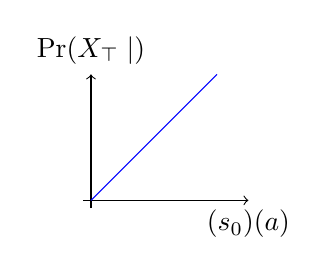
\begin{tikzpicture}[scale=2]
 \draw[->] (-0.05, 0) -- (1, 0) node[below]{$\sched(s_0)(a)$};
  	\draw[->] (0, -0.05) -- (0, 0.8) node[above] {$\Pr(X_{\lozenge\mathbf{\top}} \mid \sched)$};
  	%\draw[-,dashed] (0.4,0) -- (0.4,0.5184);
  	%\draw[-,dashed] (0.0,0.5184) -- (0.4,0.5184);
  \draw[ domain=0:0.8, smooth, variable=\x, blue] plot ({\x}, {\x});
\end{tikzpicture}
\caption{}
\end{subfigure}
\begin{subfigure}{0.38\columnwidth}
\centering
\begin{tikzpicture}[scale=2]	
 \draw[->] (-0.05, 0) -- (1, 0) node[below]{$\sched(s_0)(a)$};
  	\draw[->] (0, -0.05) -- (0, 0.8) node[above] {$H(\sched)$};
  	%\draw[-,dashed] (0.4,0) -- (0.4,0.5184);
  	%\draw[-,dashed] (0.0,0.5184) -- (0.4,0.5184);
 % \draw[ domain=0:1, smooth, variable=\x, blue] plot ({\x}, {15*(1-\x)*(1-\x)*(1-\x)*\x*\x});
\end{tikzpicture}
\caption{}
\end{subfigure}

\caption{Minimal ERCI problem.}
\end{figure}


Together, we obtain the following problem statement.
\begin{mdframed}[backgroundcolor=white!5]
\textbf{The ERCI Pareto Front Problem}:
Using the notation from the ERCI problem, find the set $\solutions \subseteq \mathbb{R}^2$.
\end{mdframed}
We are going to iteratively construct the  Pareto optimal points in $\solutions$. This yields a semi-decision procedure.
Clearly, finding $\solutions$ solves the ERCI problem, as we only need to decide whether $\langle \scthreshold, \randomness \rangle \in \solutions$.

\subsection{ERCI versus reactive control improvisation}

With these facts, we are now well-equiped to develop the algorithms in Sec.~\ref{sec:mdps} for MDPs and Sec.~\ref{sec:sgs} for SGs.

Before we continue, we compare ERCI with the reactive, i.e. 2-player control improvisation framework from~\cite{}:
\begin{mdframed}
\textbf{The Deterministic (Reactive) Control Improvisation (DCI) Problem}:
Given a \emph{deterministic} SG $\sg$, finite path sets $X_\psi$ and $X_\varphi$, and a threshold $p \in (0,1)$,  find a $\pOne$-policy $\pOneSched \in \POneScheds$  such that for every $\pTwo$-policy $\pTwoSched \in \PTwoScheds$ 
\begin{compactenum}
\item (\emph{hard constraint}) $\Pr(X_\psi \mid \sched) \geq 1$
	\item (\emph{soft constraint)} $\Pr(X_\varphi \mid \sched) \geq \scthreshold$
	\item (\emph{randomness}) $\Pr(\path) \leq \delta \text{ for all } \path \in \Paths{\sg[\sched]}$.
\end{compactenum}
\end{mdframed}
We observe that the `only' difference is that that we allow for probabilistic outcomes of actions and that we use entropy rather than an upper bound on the probability of a path. 
First, we highlight that in the reactive setting, all randomization is due to the random behavior of $\pOne$. Roughly speaking, every path is than just good (i.e., ending in a target state) or bad (i.e., ending in a sink state). The randomization criterion then may just ensure that we do not select the same path with too much probability, which intuitively means that the $\pOne$-player must ensure in every step that it selects actions where there are enough different suffixes to the path (which then means that one can uniformly randomize over these paths and meet the threshold).
In the SG case, not all paths are equal. This also directly makes the randomness constraint proposed in DIC

\begin{theorem}
	For deterministic SGs, the ERCI and DCI problem coincide.
\end{theorem}
We defer a discussion and a precise statement to Lemma~\ref{}.

\subsection{Causal Entropy versus Entropy}



%%% Local Variables:
%%% mode: latex
%%% TeX-master: "main"
%%% End:
